\documentclass{standalone}
\usepackage{tikz}
\usetikzlibrary{patterns, positioning}
\usetikzlibrary{shapes.misc}
\usepackage[outline]{contour}
\contourlength{1.5pt} 
\usepackage[sfdefault]{ClearSans} %% option 'sfdefault' activates Clear Sans as the default text font
\usepackage[T1]{fontenc}

\begin{document}
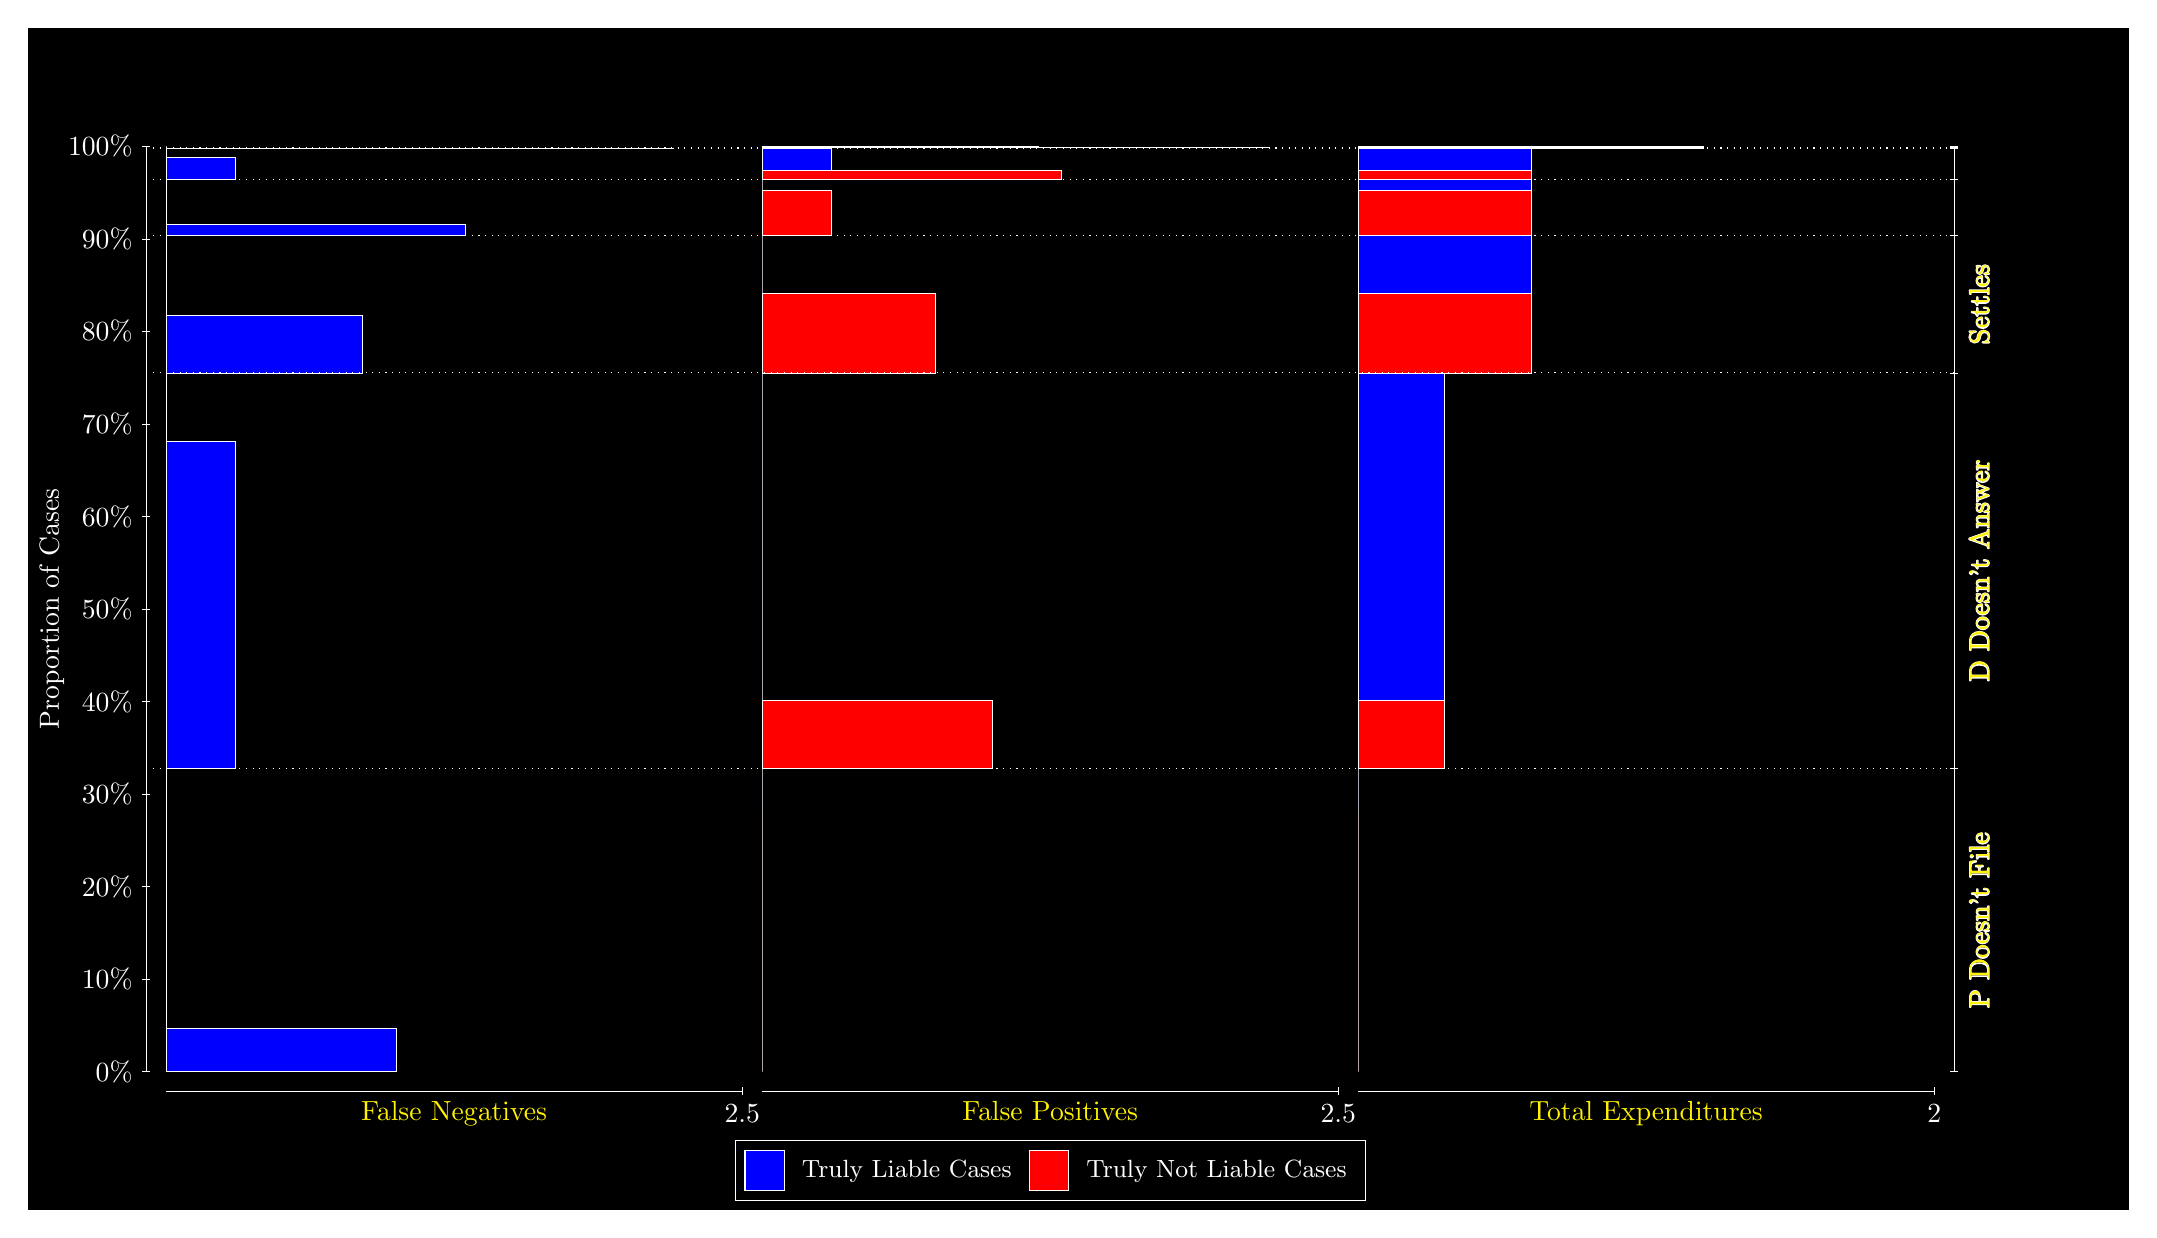
\begin{tikzpicture}
\draw[fill=black] (0,0) rectangle (26.667,15);
\draw[white, very thin] (1.5,1.75) -- (1.5,13.5);
\node[rotate=90, text=white, anchor=center] at (0.3, 7.625) {Proportion of Cases};
\draw[white, very thin] (1.45,1.75) -- (1.55,1.75);
\node[text=white, anchor=east] at (1.45, 1.75) {0\%};
\draw[white, very thin] (1.45,2.925) -- (1.55,2.925);
\node[text=white, anchor=east] at (1.45, 2.925) {10\%};
\draw[white, very thin] (1.45,4.1) -- (1.55,4.1);
\node[text=white, anchor=east] at (1.45, 4.1) {20\%};
\draw[white, very thin] (1.45,5.275) -- (1.55,5.275);
\node[text=white, anchor=east] at (1.45, 5.275) {30\%};
\draw[white, very thin] (1.45,6.45) -- (1.55,6.45);
\node[text=white, anchor=east] at (1.45, 6.45) {40\%};
\draw[white, very thin] (1.45,7.625) -- (1.55,7.625);
\node[text=white, anchor=east] at (1.45, 7.625) {50\%};
\draw[white, very thin] (1.45,8.8) -- (1.55,8.8);
\node[text=white, anchor=east] at (1.45, 8.8) {60\%};
\draw[white, very thin] (1.45,9.975) -- (1.55,9.975);
\node[text=white, anchor=east] at (1.45, 9.975) {70\%};
\draw[white, very thin] (1.45,11.15) -- (1.55,11.15);
\node[text=white, anchor=east] at (1.45, 11.15) {80\%};
\draw[white, very thin] (1.45,12.325) -- (1.55,12.325);
\node[text=white, anchor=east] at (1.45, 12.325) {90\%};
\draw[white, very thin] (1.45,13.5) -- (1.55,13.5);
\node[text=white, anchor=east] at (1.45, 13.5) {100\%};

\draw[white, very thin] (24.457,1.75) -- (24.457,13.5);
\draw[white, very thin] (24.407,1.75) -- (24.507,1.75);
\node[anchor=west] at (24.407, 1.75) {};
\draw[white, very thin] (24.407,5.5957) -- (24.507,5.5957);
\node[anchor=west] at (24.407, 5.5957) {};
\draw[white, very thin] (24.407,10.624) -- (24.507,10.624);
\node[anchor=west] at (24.407, 10.624) {};
\draw[white, very thin] (24.407,12.366) -- (24.507,12.366);
\node[anchor=west] at (24.407, 12.366) {};
\draw[white, very thin] (24.407,13.076) -- (24.507,13.076);
\node[anchor=west] at (24.407, 13.076) {};
\draw[white, very thin] (24.407,13.476) -- (24.507,13.476);
\node[anchor=west] at (24.407, 13.476) {};
\draw[white, very thin] (24.407,13.489) -- (24.507,13.489);
\node[anchor=west] at (24.407, 13.489) {};
\draw[white, very thin] (24.407,13.5) -- (24.507,13.5);
\node[anchor=west] at (24.407, 13.5) {};

\draw[white, very thin, fill=blue] (1.75,1.75) rectangle (4.6775,2.3015);
\draw[white, very thin, fill=red] (1.75,2.3015) rectangle (1.75,5.5957);
\draw[white, very thin, fill=blue] (1.75,5.5957) rectangle (2.6283,9.7495);
\draw[white, very thin, fill=red] (1.75,9.7495) rectangle (1.75,10.624);
\draw[white, very thin, fill=blue] (1.75,10.624) rectangle (4.2384,11.358);
\draw[white, very thin, fill=red] (1.75,11.358) rectangle (1.75,12.366);
\draw[white, very thin, fill=blue] (1.75,12.366) rectangle (5.5558,12.506);
\draw[white, very thin, fill=red] (1.75,12.506) rectangle (1.75,13.076);
\draw[white, very thin, fill=blue] (1.75,13.076) rectangle (2.6283,13.362);
\draw[white, very thin, fill=red] (1.75,13.362) rectangle (1.75,13.476);
\draw[white, very thin, fill=blue] (1.75,13.476) rectangle (8.1906,13.481);
\draw[white, very thin, fill=red] (1.75,13.481) rectangle (1.75,13.489);
\draw[white, very thin, fill=red] (1.75,13.489) rectangle (1.75,13.494);
\draw[white, very thin, fill=blue] (1.75,13.494) rectangle (1.75,13.5);
\draw[white, very thin, fill=red] (9.3189,1.75) rectangle (9.3189,5.0442);
\draw[white, very thin, fill=blue] (9.3189,5.0442) rectangle (9.3189,5.5957);
\draw[white, very thin, fill=red] (9.3189,5.5957) rectangle (12.246,6.4707);
\draw[white, very thin, fill=blue] (9.3189,6.4707) rectangle (9.3189,10.624);
\draw[white, very thin, fill=red] (9.3189,10.624) rectangle (11.515,11.633);
\draw[white, very thin, fill=blue] (9.3189,11.633) rectangle (9.3189,12.366);
\draw[white, very thin, fill=red] (9.3189,12.366) rectangle (10.197,12.937);
\draw[white, very thin, fill=blue] (9.3189,12.937) rectangle (9.3189,13.076);
\draw[white, very thin, fill=red] (9.3189,13.076) rectangle (13.125,13.19);
\draw[white, very thin, fill=blue] (9.3189,13.19) rectangle (10.197,13.476);
\draw[white, very thin, fill=red] (9.3189,13.476) rectangle (9.3189,13.485);
\draw[white, very thin, fill=blue] (9.3189,13.485) rectangle (9.3189,13.489);
\draw[white, very thin, fill=red] (9.3189,13.489) rectangle (15.759,13.494);
\draw[white, very thin, fill=blue] (9.3189,13.494) rectangle (12.832,13.5);
\draw[white, very thin, fill=red] (16.888,1.75) rectangle (16.888,5.0442);
\draw[white, very thin, fill=blue] (16.888,5.0442) rectangle (16.888,5.5957);
\draw[white, very thin, fill=red] (16.888,5.5957) rectangle (17.986,6.4707);
\draw[white, very thin, fill=blue] (16.888,6.4707) rectangle (17.986,10.624);
\draw[white, very thin, fill=red] (16.888,10.624) rectangle (19.083,11.633);
\draw[white, very thin, fill=blue] (16.888,11.633) rectangle (19.083,12.366);
\draw[white, very thin, fill=red] (16.888,12.366) rectangle (19.083,12.937);
\draw[white, very thin, fill=blue] (16.888,12.937) rectangle (19.083,13.076);
\draw[white, very thin, fill=red] (16.888,13.076) rectangle (19.083,13.19);
\draw[white, very thin, fill=blue] (16.888,13.19) rectangle (19.083,13.476);
\draw[white, very thin, fill=red] (16.888,13.476) rectangle (21.279,13.485);
\draw[white, very thin, fill=blue] (16.888,13.485) rectangle (21.279,13.489);
\draw[white, very thin, fill=red] (16.888,13.489) rectangle (21.279,13.494);
\draw[white, very thin, fill=blue] (16.888,13.494) rectangle (21.279,13.5);
\draw[white, dotted] (1.5,5.5957) -- (24.457,5.5957);
\draw[white, dotted] (1.5,10.624) -- (24.457,10.624);
\draw[white, dotted] (1.5,12.366) -- (24.457,12.366);
\draw[white, dotted] (1.5,13.076) -- (24.457,13.076);
\draw[white, dotted] (1.5,13.476) -- (24.457,13.476);
\draw[white, dotted] (1.5,13.489) -- (24.457,13.489);
\draw[white, very thin] (1.75,1.5) -- (9.0689,1.5);
\node[text=yellow, anchor=north] at (5.4094, 1.5) {False Negatives};
\draw[white, very thin] (9.0689,1.45) -- (9.0689,1.55);
\node[text=white, anchor=north] at (9.0689, 1.45) {2.5};

\draw[white, very thin] (9.3189,1.5) -- (16.638,1.5);
\node[text=yellow, anchor=north] at (12.978, 1.5) {False Positives};
\draw[white, very thin] (16.638,1.45) -- (16.638,1.55);
\node[text=white, anchor=north] at (16.638, 1.45) {2.5};

\draw[white, very thin] (16.888,1.5) -- (24.207,1.5);
\node[text=yellow, anchor=north] at (20.547, 1.5) {Total Expenditures};
\draw[white, very thin] (24.207,1.45) -- (24.207,1.55);
\node[text=white, anchor=north] at (24.207, 1.45) {2};

\node[text=yellow, centered, rotate=90] at (24.777, 3.6729) {\contour{white}{P Doesn't File}};
\node[text=yellow, centered, rotate=90] at (24.777, 8.1101) {\contour{white}{D Doesn't Answer}};
\node[text=yellow, centered, rotate=90] at (24.777, 11.495) {\contour{white}{Settles}};





\draw (12.978300999999998,1.5) node[draw=none] (baseCoordinate) {};
\begin{scope}[align=center]
        \matrix[scale=0.5, draw=white, below=0.5cm of baseCoordinate, nodes={draw}, column sep=0.1cm]{
            \node[rectangle, draw, minimum width=0.5cm, minimum height=0.5cm, fill=blue] {}; &
            \node[draw=none, font=\small, text=white] (B) {Truly Liable Cases}; &
            \node[rectangle, draw, minimum width=0.5cm, minimum height=0.5cm, fill=red] {}; &
            \node[draw=none, font=\small, text=white] (B) {Truly Not Liable Cases}; \\
            };
\end{scope}

\end{tikzpicture}
\end{document}